\chapter{Design und Implementierung der Partnerdatenbank}
Im Folgenden werden das Design und die Implementierung der Partnerdatenbank und die verwendeten Technologien sowie deren Implementierung beschrieben.

\section{Microservice-Architektur}
Die gesamte Applikation wird, wie in Abbildung \ref{fig:DesignOfMicroserviceArchitecture} zu sehen, als Microservice-Architektur designt. Dabei wird die Designvariante \textit{Service-Orchestrierung} gewählt. Das Partner-Service fungiert dabei als Kompositionsservice. Das Partner-Service wird dabei zur zentralen Autorität. Dies ist jedoch auch die Schwachstelle einer Microservice-Anwendung. Fällt dieses Service aus, steht die gesamte Anwendung still. Dadurch wird das Partner-Service zum \textit{Single-Point-of-Failure} in dieser Architektur. Durch das Replizieren, Skalieren und Clustering dieses Services in OpenShift kann dieses Problem einfach gelöst werden.

Wird am Frontend ein Partner- oder Unternehmens-Objekt benötigt, ruft das Frontend das Partner-Service auf. Dieses holt sich aus der PartnerDB das entsprechende Objekt und liefert dieses als Response zurück.
Werden auch die Links zu den verschiedenen Partnern benötigt, leitet das Partner-Service den Aufruf zum Docsis-Service weiter. Dieses holt sich die entsprechenden Links zum jeweiligen Partner aus der DocsisDB und liefert diese an das Partner-Service zurück. Das Partner-Service verpackt die Links in ein Partner-Objekt und liefert das Partner-Objekt an das Frontend zurück.

Werden weitere Services hinzugefügt, ruft das Partner-Service auch diese auf und liefert die Response an das Frontend zurück. In Abbildung \ref{fig:DesignOfMicroserviceArchitecture} ist zu sehen, wie das Angebotslegungs-Service in die Applikation integriert werden kann. Dieses verwaltet die Angebote in der AngebotsDB. Da die Dokumente der Angebotslegung wahrscheinlich auch in der DocsisDB gespeichert sind, könnte das Angebotslegungs-Service auch das Docsis-Service aufrufen. Um die Struktur der Anwendung so einfach wie möglich zu halten, kann auch der Umweg über das Partner-Service erfolgen. Somit redet jedes Service lediglich mit dem Partner-Service und es ist ein klarer Workflow ersichtlich.

In OpenShift wird dann lediglich die Route des Partner-Services freigegeben. Alle anderen Services kommunizieren nur intern und sind auch nur innerhalb des Clusters aufrufbar. Dadurch ist auch der Login und die Authentifizierung sowie die Autorisierung lediglich für das Partner-Service zu implementieren, da externe Clients nur Zugriff auf dieses Service haben und alle Geschäftsfälle zuerst über das Partner-Service abgewickelt werden.

\begin{figure}[H]
	\begin{center}
		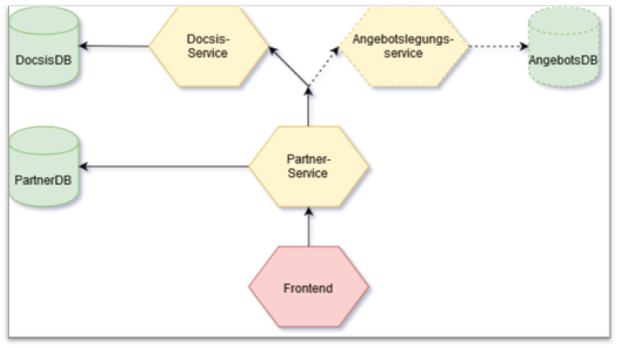
\includegraphics[scale=0.90]{DesignInOpenShift.png}
		\caption[Design der Microservice-Architektur]{Design der Microservice-Architektur}
		\label{fig:DesignOfMicroserviceArchitecture}
	\end{center}
\end{figure}

\section{Spring Boot}
Spring Boot unterstützt Entwickler bei der Erstellung von Microservice-Technologien ungemein. Spring Boot bietet dabei eine Fülle an Abhängigkeiten, die besonders für die Entwicklung von Microservices geeignet sind.

\subsection{Fehlerbehandlung mit Spring Retry}
Spring Retry bietet die Möglichkeit eine fehlgeschlagene Operation erneut ausführen zu lassen. Dies ist besonders bei REST-Aufrufen sehr wichtig. Dabei können Fehler einfacher und schneller auftreten, als wenn eine Methode eine andere Methode in derselben JVM aufgerufen werden würde. Spring Retry bietet dabei die Kontrolle über den Prozess und lässt sich einfach erweitern und anpassen \cite{SpringBootOnline}.

Bei der Verwendung von Spring Retry wird die Maven-Dependency in Listing \ref{lst:spring-retry} benötigt.
\begin{lstlisting}[language=xml, caption=pom.xml, label=lst:spring-retry]
	<dependency>
		<groupId>org.springframework.retry</groupId>
		<artifactId>spring-retry</artifactId>
	</dependency>
\end{lstlisting}

Zur Verwendung von Spring Retry muss eine Konfigurationsklasse mit \textit{@EnableRety} annotiert werden.

\subsubsection{Annotation @Retryable}
\label{ann:retryable}
\begin{lstlisting}[language=java, caption=DocsisService.java, label={lst:docsisService.retry}]
	@Retryable(value = {RestClientException.class, WebApplicationException.class},
		maxAttempts = 5,
		backoff = @Backoff(delay = 2000)
	)
	public ResponseEntity<List<Link>> getAllLinksOfPartner(Long partnerId) {
		List<Link> links = restTemplate.getForObject(restBaseServiceDocsis + 
			"links/partner/" + partnerId, ArrayList.class);
		return new ResponseEntity<>(links, HttpStatus.OK);
	}	
\end{lstlisting}

Durch den Parameter \textit{value = \{RestClientException.class, WebApplicationException.class\}} wird der Retry nur ausgeführt, wenn der Fehler vom Typ RestClientException oder WebApplicationException ist. Bei anderen Exceptions wird der Retry-Mechanismus nicht ausgelöst. 

Durch \textit{maxAttempts} kann die maximale Anzahl an Retry-Versuchen angegeben werden. Diese Methode wird bei auftretenden RestClientExceptions oder WebApplicationExceptions im Beispiel in Listing \ref{lst:docsisService.retry} maximal fünf Mal wiederholt.

Damit die Methode nicht sofort nach einem Fehlversuch neu ausgeführt wird, kann ein \textit{Backoff} angegeben werden. In diesem Fall wird zwei Sekunden nach dem Fehlversuch die Methode neu ausgeführt. \newline


\subsubsection{@Recover}
\label{ann:recover}
Eine weitere nützliche Annotation von Spring Retry ist \textit{@Recover}. Schlägt die Methode aus Listing \ref{lst:docsisService.retry} zum fünften Mal fehl, wird die Methode aus Listing \ref{lst:docsisService.recover} aufgerufen. Da sich die Behandlung bei unterschiedlichen Exceptions natürlich unterscheidet, kann die Recover-Methode auch für jede Exception explizit definiert werden. Es wird dabei automatisch die richtige Methode, die zum Typ der geworfenen Exception passt, aufgerufen.

\begin{lstlisting}[language=java, caption=DocsisService.java, label={lst:docsisService.recover}]
	@Recover
	public void recoverRestClientException(RestClientException ex){
		...
	}
	
	@Recover
	public void recoverWebApplicationException(WebApplicationException ex){
		...
	}
\end{lstlisting}

\subsubsection{Template RetryTemplate}
Spring Retry bietet auch ein Template zur generellen Konfiguration von Retry-Methoden. Im Listing \ref{lst:retryTemplate} wird eine mögliche Konfiguration von Spring Retry gezeigt.

\begin{lstlisting}[language=java, caption=RetryConfig.java, label=lst:retryTemplate]
	@Configuration
	public class RetryConfig {
		...
		@Bean
		public RetryTemplate retryTemplate() {
			RetryTemplate retryTemplate = new RetryTemplate();
			
			FixedBackOffPolicy fixedBackOffPolicy = new FixedBackOffPolicy();
			fixedBackOffPolicy.setBackOffPeriod(2000l);
			retryTemplate.setBackOffPolicy(fixedBackOffPolicy);
			
			SimpleRetryPolicy retryPolicy = new SimpleRetryPolicy();
			retryPolicy.setMaxAttempts(2);
			retryTemplate.setRetryPolicy(retryPolicy);
			
			return retryTemplate;
		}
		...
	}
\end{lstlisting}
Die \textit{RetryPolicy} bestimmt, wann oder wie oft eine Methode wiederholt werden soll. In diesem Fall zwei Mal. Die \textit{BackOffPolicy} wird zur Definition des Backoffs verwendet.

\begin{lstlisting}[language=java, caption=RetryOperations, label=lst:retryOperations]
	public interface RetryOperations {
		<T> T execute(RetryCallback<T> retryCallback) throws Exception;
		...
	}
\end{lstlisting}


Das \textit{RetryTemplate} ist eine Klasse, die das Interface RetryOperations aus Listing \ref{lst:retryOperations} implementiert. Dadurch kann das Template, wie in Listing \ref{anonymousfunction} gezeigt, aufgerufen werden.

\begin{lstlisting}[language=java, caption=Aufruf mit anonymer Funktion, label=anonymousfunction]
	retryTemplate.execute(new RetryCallback<Void, RuntimeException>() {
		@Override
		public Void doWithRetry(RetryContext arg0) {
			myService.templateRetryService();
			...
		}
	});
\end{lstlisting}

Alle Methoden innerhalb der \textit{doWithRetry}-Methode unterliegen nun der Spezifikation von RetryConfig.
Der Aufruf kann natürlich auch einfacher mit einer Lambda-Expression statt einer anonymen Funktion erfolgen (Listing \ref{lst:lambda}).

\begin{lstlisting}[language=java, caption=Aufruf mittels Lambda-Expression, label=lst:lambda]
	retryTemplate.execute(arg0 -> {
		myService.templateRetryService();
		...
	});
\end{lstlisting}


\subsection{REST-Schnittstellenbeschreibung mit Swagger}
Gerade bei Microservice-Applikationen ist es essenziell, passende Spezifikationen und Dokumentationen für die REST-Schnittstellen zu erstellen. Diese Dokumentationen sollten informativ, lesbar und einfach zu folgen sein. 

Wird diese Dokumentation manuell erstellt, werden oft Änderungen in der API nicht sofort in der Dokumentation nachgezogen. Dies ist natürlich für Aufrufer der API und Anwender des Services fatal, da Aufrufe plötzlich nicht mehr funktionieren und es scheinbar keine Änderungen gab.

Dieses Problem löst Swagger. Swagger ist ein Tool zur automatischen Dokumentation der REST-API. Dadurch ist die Dokumentation stets aktuell.

In der Partnerdatenbank wird die Springfox Implementierung von Swagger verwendet. Dazu wird die Maven-Dependency in Listing \ref{lst:springfox-swagger} benötigt.
\begin{lstlisting}[language=xml, caption=pom.xml, label=lst:springfox-swagger]
	<dependency>
		<groupId>io.springfox</groupId>
		<artifactId>springfox-swagger2</artifactId>
	</dependency>
\end{lstlisting}


Swagger wird durch die Annotation \textit{@EnableSwagger2} aktiviert. Das Docket-Bean muss definiert werden. Die \textit{select}-Methode des Docket-Beans liefert eine Instanz der Klasse \textit{ApiSelectorBuilder} zurück. Diese bietet einen Weg, um die Endpoints von Swagger zu kontrollieren. Durch die \textit{RequestHandlerSelections} wird angegeben, dass lediglich REST-Methoden im Basispaket \glqq at.fh.se.master.company\grqq{} durch Swagger dokumentiert werden.
\begin{lstlisting}[language=java, caption=Swagger-Konfiguration, label=lst:swaggerconf]
	@SpringBootApplication
	@EnableSwagger2
	public class CompanyServiceApplication {
		...
		@Bean
		public Docket productApi() {
			return new Docket(DocumentationType.SWAGGER_2)
			.select()
			.apis(
				RequestHandlerSelectors
					.basePackage("at.fh.se.master.company")
			).build();
		}
		...
	}
\end{lstlisting}

Die Swagger-Dokumentation ist nach dem Start der Applikation unter dem Link \textit{http://localhost:8080/spring-security-rest/api/v2/api-docs} erreichbar. Dies ist ein JSON-Objekt mit Key-Value Paaren. Diese Datei ist leider für Menschen nicht gut lesbar.
Springfox bietet daher mit der Maven-Dependency aus Listing \ref{lst:springfoxswaggerui} eine UI zur besseren Darstellung der REST-Methoden:

\begin{lstlisting}[language=xml, caption=pom.xml, label=lst:springfoxswaggerui]
	<dependency>
		<groupId>io.springfox</groupId>
		<artifactId>springfox-swagger-ui</artifactId>
	</dependency>
\end{lstlisting}

Die UI ist nach dem Starten der Applikation unter \textit{http://localhost:8080/swagger-ui.html} erreichbar. Sie zeigt alle REST-Methoden der Applikation in einer grafischen Darstellung. Mit dieser UI können die einzelnen REST-Methoden auch aufgerufen und getestet werden.

\subsection{Tracing mit Jaeger}
\label{sec:tracingwithjaeger}
Jaeger ist eine Applikation zum Tracen von Serviceaufrufen in Anwendungen. Bei der Implementierung einer Microservice-Architektur treten viele Probleme und Hürden auf. Diese Probleme betreffen hauptsächlich die beiden Gebiete \textbf{Netzwerke} und \textbf{Aufspürbarkeit von Services}. Es ist sehr viel komplexer, ein System bestehend aus kleinen Untersystemen zu debuggen als eine einzelne Applikation \cite{jaeger}.

Jaeger addressiert dabei folgende Probleme \cite{jaeger}:
\begin{itemize}
	\item Verteiltes Monitoring von Transaktionen.
	\item Performanz- und Latenzoptimierungen.
	\item Ursachenanalyse.
	\item Analyse der Serviceabhängigkeiten.
	\item Verteilte Propagierung von Kontexten.
\end{itemize}

Folgenden Features bietet Jaeger, um die Nutzung noch einfacher zu machen \cite{jaeger}:
\begin{itemize}
	\item \textbf{Hohe Skalierbarkeit}: Das Jaeger-Backend besitzt keinen Single-Point-of-Failure und skaliert mit den Businessanforderungen. Dies ist gerade bei der Entwicklung von Microservices von großer Bedeutung.
	\item \textbf{Nativer Support für OpenTracing}: Das Jaeger Backend, die Web UI und die Bibliotheken von Jaeger sind so designt, dass sie von Grund auf den OpenTracing-Standard unterstützen. Dazu gehören:
	\begin{itemize}
		\item das repräsentieren der Traces als direkte azyklische Graphen über Span-Referenzen,
		\item der Support von typisierten Span Tags und strukturierten Logs,
		\item der Support von verteilter Kontextpropagierung.
	\end{itemize}
	\item \textbf{Mehrere Speicher-Backends}: Jaeger unterstützt zwei populäre OpenSource NoSQL-Datenbanken als Speicher-Backends: Cassandra und Elasticsearch. Jaeger enthält auch einen In-Memory-Speicher für Test-Setups.
	\item \textbf{Modernes Web UI}: Die Jaeger Web UI wurde mit JavaScript und React entwickelt. Verschiedene Performanzverbesserungen wurden im Laufe der Jahre eingebaut, um tausende Spans zu tracen.
	\item \textbf{Cloud-Native Deployment}: Das Jaeger Backend besteht aus einer Sammlung von Docker-Containern. Das Deployment zum Kubernetes-Cluster wird durch \textit{Kubernetes Operators}, \textit{Kubernetes Templates} und \textit{Helm Charts} vereinfacht.
	\item \textbf{Beobachtbarkeit}: Alle Jaeger-Backend-Komponenten bieten standardmäßig Metriken an. Logs werden dabei mittels strukturiertem Logging auf der Konsole ausgegeben.
	\item \textbf{Rückwärtskompatibilität mit Zipkin}: Sofern bestehende Anwendungen Bibliotheken von Zipkin Web-Versionen verwenden, sind diese auch mit Jaeger kompatibel. Anwendungen, die bereits mit Zipkin getraced werden, müssen daher nicht neu geschrieben werden.
\end{itemize}

Auch für Jaeger gibt es eine UI zur Darstellung der Serviceaufrufe. Um die \textit{JaegerUI}, den \textit{collector}, die \textit{query} und den \textit{agent} inklusive einer Speicherkomponente zu starten, kann folgender Docker-Befehl in der Kommandozeile ausgeführt werden:

\begin{lstlisting}
$ docker run -d --name jaeger \
	-e COLLECTOR_ZIPKIN_HTTP_PORT=9411 \
	-p 5775:5775/udp \
	-p 6831:6831/udp \
	-p 6832:6832/udp \
	-p 5778:5778 \
	-p 16686:16686 \
	-p 14268:14268 \
	-p 14250:14250 \
	-p 9411:9411 \
	jaegertracing/all-in-one:1.17
\end{lstlisting}
Dieser Befehl startet einen Docker Container aus dem Docker Image \textit{jaegertracing/all-in-one:1.17} und gibt die entsprechenden Ports frei. Diese Applikation kann nun unter der URL \textit{http://localhost:16686} aufgerufen werden und kann Traces über die entsprechenden Ports entgegennehmen.

Für die Verwendung von Jaeger in einer Spring Boot-Applikation muss die Maven-Dependency aus Listing \ref{opentracing-spring-jaeger} hinzugefügt werden.
\begin{lstlisting}[language=xml, caption=pom.xml, label=opentracing-spring-jaeger]
	<dependency>
		<groupId>io.opentracing.contrib</groupId>
		<artifactId>opentracing-spring-jaeger-cloud-starter</artifactId>
	</dependency>
\end{lstlisting}


\begin{lstlisting}[language=yml, caption=application.yml, label=lst:jaeger.params]
	spring:
		application:
			name: partner-service
	opentracing:
		jaeger:
			udp-sender:
				host: localhost
				port: 6831
\end{lstlisting}

Um die JaegerUI lokal erreichen zu können, müssen im \textit{application.yml} zumindest die in Listing \ref{lst:jaeger.params} gezeigten Parameter angegeben werden. Die Traces dieser Applikation werden nun unter dem Namen \glqq partner-service\grqq{} angezeigt.
Der \textit{host}- und der \textit{port}-Parameter geben den Endpoint der Jaeger-CLI, hinter der der Collector sitzt.

Für das Deployment der JaegerUI in OpenShift steht ein Template zur Verfügung. Mit folgendem Befehl kann die JaegerUI einfach deployt werden:
\begin{lstlisting}[language=bash]
$ 	oc process -f jaeger-all-in-one-template.yml | oc create -f -
\end{lstlisting}

Dadurch verarbeitet OpenShift das Template und erstellt auch die Applikation. Auch die Route wird freigegeben und die JaegerUI ist im Browser erreichbar.
Für die Verwendung der JaegerUI in OpenShift müssen in der Datei \textit{application.yml} die Parameter wie in Listing \ref{lst:jaeger.params.openshift} geändert werden.
\begin{lstlisting}[language=yml, caption=application.yml, label=lst:jaeger.params.openshift]
spring:
	application:
		name: partner-service
opentracing:
	jaeger:
		udp-sender:
			host: jaeger-agent
			port: 6831
\end{lstlisting}

Dadurch werden die Traces an die JaegerUI im selben Cluster wie die Anwendung gesendet.

Grundsätzlich werden alle REST-Methoden getract, es kann jedoch mit der Annotation \textit{@Traced} eine Methode ausgeschlossen werden.
\begin{lstlisting}[language=java, caption=LinkControllerApi.java, label=TracedAnnotation]
	@RequestMapping("/")
	@Traced(false)
	public interface LinkControllerApi {
		ResponseEntity<List<Link>> getAllLinksOfPartner(@PathVariable("id") 
			Long partnerId);
		
		@Traced(true)
		ResponseEntity addLink(@RequestBody @NotNull @Valid Link link);
		
		ResponseEntity deleteLink(@PathVariable Long id);
	}
\end{lstlisting}

Die Annotation @Traced kann auch auf Klassenebene hinzugefügt werden. Dadurch sind alle Methoden dieser Klasse betroffen. Durch dieselbe Annotation auf Methodenebene kann eine bestimmte Methode aus der Konfiguration der Klassenebene ausgenommen werden. In Listing \ref{TracedAnnotation} wird dadurch lediglich die Methode \textit{addLink} getract.

\subsection{Spring Boot Actuator}
Spring Boot stellt mit dem Actuator-Modul eine breite Palette zum Monitoring und Managen einer Spring Boot Applikation zur Verfügung. Durch das Actuator-Modul können Features, wie Health-Checks, Auditing, Sammeln von Metrics oder HTTP-Tracing, einfach bereitgestellt werden. Auf diese Features kann über JMX- oder HTTP-Endpoints zugegriffen werden. 

Zur Verwendung von Spring Boot Actuator muss die Maven-Dependency aus Listing \ref{actuator.dependency} hinzugefügt werden.
\begin{lstlisting}[language=xml, caption=pom.xml, label=actuator.dependency]
	<dependency>
		<groupId>org.springframework.boot</groupId>
		<artifactId>spring-boot-starter-actuator</artifactId>
	</dependency>
\end{lstlisting} 

Die verschiedenen Endpoints können im \textit{application.yml} aktiviert werden. Dazu muss die Environment-Variable \textbf{management.endpoint.<endpoint>.enabled} auf \textbf{true} gesetzt werden. Der Wert \textit{<endpoint>} ist dabei ein Platzhalter für z.B. den Endpoint \textit{info} oder \textit{health}.

Folgende Endpoints stehen zur Verfügung:
\begin{itemize}
	\item \textbf{auditevents}: Gibt Auditevents, wie \textit{auth\_success} oder \textit{order\_success} der Applikation nach außen frei.
	\item \textbf{info}: Gibt grundsätzliche Informationen über die Applikation frei. 
	\item \textbf{health}: Zeigt den Health-Status der Applikation an.
	\item \textbf{metrics}: Gibt Metric-Informationen nach außen frei. Misst z.B. wie oft eine REST-Schnittstelle aufgerufen wurde und wie lange ein Aufruf durchschnittlich dauert.
	\item \textbf{loggers}: Zeigt die konfigurierten Logger an.
	\item \textbf{logfile}: Gibt den Inhalt des Logfiles aus.
	\item \textbf{httptrace}: Zeigt Trace-Informationen über die letzten 100 HTTP-Requests und HTTP-Responses an.
	\item \textbf{env}: Zeigt die derzeit konfigurierten Environment-Variablen an.
	\item \textbf{shutdown}: Fährt die Applikation herunter.
	\item \textbf{mappings}: Zeigt eine Liste zu allen @RequestMapping-Pfaden. 
	\item \textbf{scheduledtasks}: Zeigt eine Liste aller Scheduled Tasks an.
	\item \textbf{threaddump}: Führt einen Thread Dump aus.
	\item \textbf{heapdump}: Gibt einen JVM Heap Dump zurück.
\end{itemize}

Der wichtigste Endpoint in Verbindung mit dem Deployment der Applikation in OpenShift ist der \textit{Health}-Endpoint. OpenShift prüft mit der \textit{ReadinessProbe} und der \textit{LivenessProbe} ob die Applikation im Container noch verfügbar ist. Ist dies nicht der Fall, wird auch der Pod heruntergefahren.

Der Health-Endpoint ist, sofern aktiviert, unter der URL \textit{/actuator/health} erreichbar. Dieser liefert lediglich die JSON-Response aus Listing \ref{json} und den Status 200 zurück:
\begin{lstlisting}[language=json, caption=Healt-Endpoint, label=json]
	{
		"status": "UP"
	}
\end{lstlisting}

OpenShift prüft bei der \textit{ReadinessProbe} und der \textit{LivenessProbe} lediglich auf den Status 200. 

Metriken, Traces und Health-Checks sind gerade beim Einsatz von Microservices von großer Bedeutung, um sicherzugehen, dass die einzelnen Microservices laufen, und um Fehlerfälle auch über Servicegrenzen hinweg nachverfolgen zu können.

\section{Automatisierte Test-, Build- und Deployment-Pipelines mit Jenkins}
Die Definition der Pipelines wird in der Datei \textit{maven-pipeline.yml} angegeben. In dieser Datei befinden sich die folgenden Definitionen für OpenShift-Objekte:
\begin{enumerate}
	\item Template,
	\item ImageStream,
	\item BuildConfig,
	\item DeploymentConfig,
	\item Service,
	\item Route.
\end{enumerate}

Diese Objekte werden im Folgenden näher erklärt.

\subsection{Template}
Im Template können Parameter gesetzt werden, die danach in der gesamten \textit{maven-pipeline.yml}-Datei verwendet werden können. Dadurch müssen bei Änderungen lediglich diese Werte geändert werden und nicht in der gesamten Datei nachgezogen werden. Der Parameter \textit{APP\_NAME} kann in der Datei durch den Ausdruck \textit{\$\{APP\_NAME\}} verwendet werden. 

\subsection{ImageStream}
Im ImageStream werden das zu referenzierende Image und der ImageStreamTag angegeben. Dies wird durch die beiden \textit{from}-Befehle im Listing \ref{maven-pipeline} angegeben:
\begin{lstlisting}[language=yml, caption=maven-pipeline.yml - Template, label=maven-pipeline]
	apiVersion: v1
	kind: ImageStream
	name: "jdk-11"
	spec:
		tags:
			from:
				kind: DockerImage
				name: registry.access.redhat.com/openjdk/openjdk-11-rhel7:latest
			from:
				kind: ImageStreamTag
				name: "jdk-11"
\end{lstlisting}

Dadurch wird das Docker Image mit dem Tag \textit{jdk-11} in der OpenShift internen Registry markiert.

\subsection{BuildConfig}
In der Datei \textit{maven-pipeline.yml} werden zwei BuildConfigs definiert. Die erste führt den Jenkins Build am Jenkins Build Server aus und die zweite definiert das Docker Image, mit dem die Applikation gebaut und gestartet wird.

\subsubsection{Jenkins Build}
In Listing \ref{lst:jenkinsPipelineStrategy} ist die die BuildConfig-Definition für den Jenkins Build zu sehen.

\begin{lstlisting}[language=yml, caption=maven-pipeline.yml - Jenkins BuildConfig, label=lst:jenkinsPipelineStrategy]
	apiVersion: v1
	kind: BuildConfig
	metadata:
		name: ${APP_NAME}
	spec:
		strategy:
			jenkinsPipelineStrategy:
				jenkinsfile: |-
					try {
						timeout(time: 40, unit: 'MINUTES') {
							def appName="partner-service"
							def project=""
							
							node {
								stage("Initialize") {
									project = env.PROJECT_NAME
								}
							}
							
							node("maven") {
								stage("Checkout") {
									git url: ${GIT_URL}, branch: "master"
								}
								stage("Build WAR") {
									sh "mvn clean package -f
										src/Partnerdatenbank/partner-service/pom.xml"
									stash name:"war", includes:
										"src/Partnerdatenbank/partner-service/target/*"
								}
							}
							
							node {
								stage("Build Image") {
									dir("war") {
										unstash name:"war"
									}
									sh "oc start-build ${appName}-docker --from-file=war/src/
											Partnerdatenbank/partner-service/target/
												partner-service-0.0.1-SNAPSHOT.jar -n ${project}"
									timeout(time: 40, unit: 'MINUTES') {
										openshift.withCluster() {
											openshift.withProject() {
												def bc = openshift.selector('bc', "${appName}-docker")
												echo "Found 1 ${bc.count()} buildconfig"
												def blds = bc.related('builds')
												blds.untilEach {
													return it.object().status.phase == "Complete"
												}
											}
										}  
									}
								}
								stage("Deploy") {
									openshift.withCluster() {
										openshift.withProject() {
											def dc = openshift.selector('dc', "${appName}")
											dc.rollout().status()
										}
									}
								}
							}
						}
					} catch (err) {
						echo "in catch block"
						echo "Caught: ${err}"
						currentBuild.result = 'FAILURE'
						throw err
					}
				type: JenkinsPipeline
\end{lstlisting}

Durch den Parameter \textit{jenkinsPipelineStrategy} wird die Build-Strategie \textit{Pipeline Build} verwendet. Bei der ersten Pipeline mit dieser Strategie instanziert OpenShift einen Jenkins-Server, der die Pipelines ausführt. Weitere Pipelines verwenden diesen Jenkins-Server.

Die Definitionen im \textit{jenkinsfile}-Segment können auch in einem eigenen Jenkinsfile definiert werden. Im \textit{maven-pipeline.yml} muss darauf referenziert werden.

Im Folgenden werden die einzelnen Segmente des Jenkinsfiles beschrieben:
\begin{enumerate}
	\item \textbf{timeout}: Der Timeout bestimmt die maximale Dauer der Ausführung der Pipeline. Überschreitet der Build inklusive dem Deployment 40 Minuten, wird der Build abgebrochen.
	\item \textbf{stage(\grqq Initialize\grqq)}: In dieser Stage wird der Variablen \textit{project} der Projektname zugewiesen. Dadurch ist er in der Datei verwendbar.
	\item \textbf{node(\grqq maven\grqq)}: In diesem Abschnitt wird der Masterbranch des Git-Repository ausgecheckt. Danach wird die Applikation gebaut und das angegebene Verzeichnis im Git-Repository gestasht. \textit{Git stash} speichert die Änderungen in diesem Verzeichnis und stellt das ursprüngliche Git-Repository wieder her, falls andere Änderungen am Repository durch den Build vorgenommen wurden.
	\item \textbf{stage(\grqq Build Image\grqq)}: In dieser Stage erfolgt das unstashen des Git-Repository. Auch das Bauen der Applikation in OpenShift mit der vorher gebauten \textit{jar}-Datei findet in dieser Stage statt. Dazu wird ein Dockerfile benötigt. Dieses ist in der zweiten BuildConfig integriert.
	\item \textbf{stage(\grqq Deploy\grqq)}: In dieser Stage findet das Deployment der Applikation im Cluster im angegebenen Projekt statt. 
\end{enumerate}

\subsubsection{Docker Build}
In Listing \ref{lst:DockerPipelineStrategy} ist die BuildConfig-Definition für den Docker Build zu sehen.

\begin{lstlisting}[language=yml, caption=maven-pipeline.yml - Docker BuildConfig, label=lst:DockerPipelineStrategy]
	apiVersion: v1
	kind: BuildConfig
	metadata:
		labels:
		name: ${APP_NAME}-docker
	spec:
		output:
		to:
			kind: ImageStreamTag
			name: ${APP_NAME}:latest
	source:
		dockerfile: |-
			FROM registry.access.redhat.com/openjdk/openjdk-11-rhel7:latest
			COPY partner-service-0.0.1-SNAPSHOT.jar 
				/partner-service-0.0.1-SNAPSHOT.jar
			EXPOSE 8080
			ENTRYPOINT exec java -jar 
				/partner-service-0.0.1-SNAPSHOT.jar
		binary:
			asFile: partner-service-0.0.1-SNAPSHOT.war
		type: Docker
	strategy:
		dockerStrategy:
			from:
				kind: ImageStreamTag
				name: openjdk-11-rhel7:latest
		type: Docker
\end{lstlisting}

Durch diese BuildConfig wird das Dockerfile definiert, das für den Jenkins Build benötigt wird. Das Dockerfile selbst ist sehr einfach gehalten und nimmt das Docker Image \textit{openjdk-11-rhel7} als Basis Image. Das gebaute jar wird in den Container kopiert und der Port 8080 freigegeben. Durch den Entrypoint wird die Applikation im Container gestartet.

\subsection{DeploymentConfig}
In Listing \ref{deploymentConfig} wird der DeploymentConfig-Abschnitt gezeigt.
\begin{lstlisting}[language=yml, caption=maven-pipeline.yml - DeploymentConfig, label=deploymentConfig]
	apiVersion: v1
	kind: DeploymentConfig
	metadata:
		labels:
			name: ${APP_NAME}
	spec:
		replicas: 1
		selector:
			app: ${APP_NAME}
			deploymentconfig: ${APP_NAME}
		strategy:
			rollingParams:
				intervalSeconds: 1
				maxSurge: 25%
				maxUnavailable: 25%
				timeoutSeconds: 600
				updatePeriodSeconds: 1
			type: Rolling
	template:
		spec:
			containers:
				- image: ${APP_NAME}:latest
				imagePullPolicy: Always
				name: ${APP_NAME}
				ports:
				  - containerPort: 8080
					protocol: TCP
				resources: {}
				terminationMessagePath: /dev/termination-log
				livenessProbe:
					httpGet:
						path: /actuator/health
						port: 8080
						scheme: HTTP
					initialDelaySeconds: 10
					timeoutSeconds: 2
					periodSeconds: 10
					successThreshold: 1
					failureThreshold: 3
				readinessProbe:
					httpGet:
						path: /actuator/health
						port: 8080
						scheme: HTTP
					initialDelaySeconds: 30
					timeoutSeconds: 2
					periodSeconds: 10
					successThreshold: 1
					failureThreshold: 3
	triggers:
	  - type: ConfigChange
	  - imageChangeParams:
			automatic: true
			containerNames:
		      - ${APP_NAME}
			from:
				kind: ImageStreamTag
				name: ${APP_NAME}:latest
		type: ImageChange
\end{lstlisting}

In der DeploymentConfig wird definiert, wie das Deployment des Pods erfolgt. Auch die ReadinessProbe und die LivenessProbe werden hier definiert.

Im Folgenden werden die wichtigsten Segmente des DeploymentConfig-Abschnittes beschrieben:
\begin{itemize}
	\item \textbf{strategy}: Beim Deployment eines Pods stehen zwei verschiedene Strategien zur Verfügung.
	\begin{enumerate}
		\item \textbf{Rolling}: Bei der Rolling-Strategie wird zuerst der neue Pod hochgefahren und erst danach der alte Pod gelöscht. Dadurch entsteht keine Downtime der Applikation. Diese ist somit immer verfügbar.
		\item \textbf{Recreate}: Bei der Recreate-Strategie wird der alte Pod gelöscht und erst nach dem Löschen der neue Pod hochgefahren. Dies wird benötigt, wenn eine Applikation den alten Stand und den neuen Stand gleichzeitig nicht unterstützt. Dies kann bei Breaking Changes der Fall sein.
	\end{enumerate}
	\item \textbf{livenessProbe}: Mit der Liveness-Probe überprüft OpenShift in Intervallen, ob die Applikation noch läuft. Dadurch muss ein REST-Aufruf angegeben werden. Diesen ruft OpenShift auf und erwartet den Response Status 200. Durch \textit{successThreshold} und \textit{failureFreshold} kann angegeben werden, wann OpenShift den Pod herunterfährt, sobald die Applikation nicht mehr erreichbar ist.
	\item \textbf{readinessProbe}: Während dem Deployment überprüft OpenShift ob die Applikation bereits fertig deployt und gestartet wurde. Auch hier muss ein REST-Endpoint für den Aufruf angegeben werden.
	\item \textbf{triggers}: Durch Trigger kann ein automatischer Rebuild und Redeploy der Applikation angegeben werden. Sobald sich das Image ändert, baut und deployt OpenShift diese Applikation neu. 
\end{itemize}

\subsection{Service}
Durch die Service-Definition wird der Name des Services und der Port, hinter dem die Applikation läuft, angegeben. Die Definition des Services sieht, wie in Listing \ref{Service} gezeigt, aus.

\begin{lstlisting}[language=yml, caption=maven-pipeline.yml - Servicem, label=Service]
	apiVersion: v1
	kind: Service
	metadata:
		labels:
			name: ${APP_NAME}
	spec:
		ports:
		  - name: 8080-tcp
			port: 8080
			protocol: TCP
			targetPort: 8080
		selector:
			app: ${APP_NAME}
			deploymentconfig: ${APP_NAME}
		sessionAffinity: None
		type: ClusterIP
\end{lstlisting}

\subsection{Route}
Durch die Definition der Route wird diese nach außen frei gegeben. Das Service ist dadurch von externen Clients erreichbar. Die Definition der Route sieht, wie in Listing \ref{Route} gezeigt, aus:

\begin{lstlisting}[language=yml, caption=maven-pipeline.yml - Service, label=Route]
	apiVersion: v1
	kind: Route
	metadata:
		labels:
			name: ${APP_NAME}
	spec:
		to:
			kind: Service
			name: ${APP_NAME}
	port:
		targetPort: 8080-tcp
	wildcardPolicy: None
\end{lstlisting}

\subsection{Starten der Pipeline}
Diese Pipeline kann über die Web Console oder über die CLI mit folgendem Befehl erfolgen:
\begin{lstlisting}[language=bash]
$	oc create -f maven-pipeline.yml
\end{lstlisting}

Dadurch startet OpenShift einen Jenkins-Server, der die Tests ausführt und das Bauen der Applikation übernimmt. Die Applikation wird in OpenShift deployt und danach die Route freigegeben. Dadurch ist das Service unter der angegebene Route verfügbar und kann auch von externen Clients verwendet werden.


\section{Environment-Variablen in OpenShift}
Environment-Variablen in OpenShift werden durch \textit{ConfigMaps} und \textit{Secrets} definiert. Dadurch müssen diese Variablen nicht in der Applikation selbst verwaltet werden.

\subsection{ConfigMaps}
Ein ConfigMap-Objekt bietet einen Mechanismus, um Konfigurationsdaten in Container injizieren zu können. Ein ConfigMap-Objekt hält Key-Value-Paare der Konfigurationsdaten, die von den Pods oder Controllern genutzt werden können. Ein ConfigMap-Objekt verhält sich ähnlich zu einem Secret (siehe Abschnitt \ref{subsubsec:secrets}). In einer ConfigMap werden jedoch keine sensiblen Daten gespeichert \cite{OpenShiftOnline}.

Die ConfigMap-Definition für die Partnerdatenbank sieht, wie in Listing \ref{configmap} gezeigt, aus:
\begin{lstlisting}[language=yml, caption=partnerdatenbank-config.yml, label=configmap]
	apiVersion: v1
	kind: ConfigMap
	data:
		DATABASE_NAME: mssql
		DATABASE_PORT: "1433"
		DATABASE_SERVICE_DOCSIS: DocsisDB
		DATABASE_SERVICE_PARTNER: PartnerDB
		SERVICE_DOCSIS_NAME: 
			"http://docsis-service-partnerdatenbank.10.0.75.2.nip.io"
		SERVICE_DOCSIS_PORT: "8080"
		SERVICE_PARTNER_PORT: "8080"
		SERVICE_JAEGER_HOST: jaeger-agent
		SERVICE_JAEGER_PORT: "6831"
	metadata:
		name: partnerdatenbank-config
		namespace: partnerdatenbank
\end{lstlisting}

In dieser Datei werden die Zugriffsdaten zur Datenbank und Daten über die einzelnen Microservices gehalten. Auch der Host und Port der JaegerUI wird in der ConfigMap definiert.
Über folgenden Befehl kann die ConfigMap in OpenShift erstellt werden:
\begin{lstlisting}[language=bash]
$	oc create -f partnerdatenbank-config.yml
\end{lstlisting}

Dadurch sind diese Environment-Variablen in OpenShift verfügbar. 

Die Verwendung in der Applikation wird in Listing \ref{lst:ConfigmapUsage} gezeigt.
\begin{lstlisting}[language=yml, caption=application.yml - ConfigMap, label=lst:ConfigmapUsage]
	spring:
		profiles: openshift
		datasource:
			url: jdbc:sqlserver://${DATABASE_NAME}:${DATABASE_PORT};
				databaseName=${DATABASE_SERVICE_PARTNER}
			username: ${DATABASE_USERNAME}
			password: ${DATABASE_PASSWORD}
	base:
		service:
		docsis: ${SERVICE_DOCSIS_NAME}/
	opentracing:
		jaeger:
			udp-sender:
				host: ${SERVICE_JAEGER_HOST}
				port: ${SERVICE_JAEGER_PORT}
\end{lstlisting}

Diese Konfigurationdaten können auch zur Laufzeit geändert werden. Sie müssen jedoch beim Start einer Applikation verfügbar sein. Injiziert eine Applikation einen Parameter, der nicht verfügbar ist, schlägt das Deployment fehl. 
ConfigMaps können lediglich von Containern im selben Namespace genutzt werden. 

\subsection{Secrets}
\label{subsubsec:secrets}
Das Speichern von sensiblen Daten, wie Zugriffsdaten auf eine Datenbank in der Applikation selbst, ist sehr gefährlich. Oft werden Projekte in öffentlichen Git-Repositories gehalten und jeder hat Zugriff darauf. 

Secrets sind ein Mechanismus zur Behandlung von sensiblen Daten in OpenShift. Secrets entkoppeln sensible Informationen von Pods. Secrets können in den Pod gemountet werden.

Die Definition des Secrets für die Partnerdatenbank sieht wie folgt aus:
\begin{lstlisting}[language=yml, caption=partnerdatenbank-secret-config.yml]
	apiVersion: v1
	kind: Secret
	stringData:
		DATABASE_USERNAME: <username>
		DATABASE_PASSWORD: <password>
	metadata:
		name: partnerdatenbank-secret-config
		namespace: partnerdatenbank
\end{lstlisting}

Hierbei sind der Parameter \textit{<username>} und \textit{<password>} lediglich Platzhalter für die eigentlichen sensiblen Daten, die in dieser Arbeit nicht gezeigt werden. Secrets werden in base64 konvertiert und gespeichert.

In dieser Datei werden die Zugangsdaten für die Datenbank gehalten. Mit folgendem Befehl werden Secrets in OpenShift erstellt:
\begin{lstlisting}[language=bash]
$ 	oc create -f partnerdatenbank-secret-config.yml
\end{lstlisting}

Dadurch können diese von Pods und Controller genutzt werden. Auch Secrets liegen in einem Namespace und können lediglich innerhalb dieses Namespaces erreicht werden.
Die Verwendung der Secrets in der Applikation kann in Listing \ref{lst:ConfigmapUsage} bei den Parametern \textit{username} und \textit{password} betrachtet werden.


\section{Deployment in OpenShift mit dem fabric8-maven-plugin}
Das \textbf{fabric8-maven-plugin} hilft beim Deployment der Applikation in OpenShift. Das fabric8-maven-plugin  fokussiert auf folgende zwei Aufgaben:
\begin{enumerate}
	\item Erstellen von Docker Images,
	\item Erstellen von OpenShift Ressource Deskriptoren.
\end{enumerate}

Das Plugin kann sehr flexibel konfiguriert werden und bietet mehrere Konfigurationsmöglichkeiten für das Deployment. Das Plugin für die Partnerdatenbank wird wie in Listing \ref{properties} konfiguriert.

\begin{lstlisting}[language=xml, caption=pom.xml - fabric8-maven-plugin, label=properties]
	
	<properties>
		<fabric8-maven-plugin.version>4.4.0</fabric8-maven-plugin.version>
		
		...
		
		<fabric8.mode>openshift</fabric8.mode>
		<fabric8.generator.fromMode>docker</fabric8.generator.fromMode>
		<fabric8.generator.from>
			registry.access.redhat.com/openjdk/openjdk-11-rhel7:latest
		</fabric8.generator.from>
	</properties>
	
	...
	
	<profile>
		<id>openshift</id>
		<build>
			<plugins>
				<plugin>
					<groupId>io.fabric8</groupId>
					<artifactId>fabric8-maven-plugin</artifactId>
					<version>${fabric8-maven-plugin.version}</version>
					<executions>
						<execution>
							<id>fmp</id>
							<goals>
								<goal>resource</goal>
								<goal>build</goal>
							</goals>
						</execution>
					</executions>
				</plugin>
			</plugins>
		</build>
	</profile>
	
	...
\end{lstlisting}

Durch die \textbf{fabric8.<parameter>}-Properties kann das Plugin konfiguriert werden.
Im Folgenden werden die definierten Properties näher beschrieben:

\begin{itemize}
	\item \textbf{fabric8.mode}: Der mode-Parameter bestimmt den Buildmodus. Dieser Parameter kann drei verschiedene Werte annehmen:
	\begin{enumerate}
		\item \textit{Kubernetes}: Erstellt ein Docker Image durch den Docker Daemon.
		\item \textit{OpenShift}: Triggert einen OpenShift Build. Dieser kann entweder ein S2I-Build oder ein Docker Binary Build sein. Diese hängt vom Property fabric8.buildStrategy ab.
		\item \textit{auto}: Dadurch wird der Modus von fabric8 durch den konfigurierten Cluster erkannt. Dieser Parameter ist standardmäßig eingestellt.
	\end{enumerate}
	\item \textbf{fabric8.generator.fromMode}: Wenn ein S2I-Build konfiguriert ist, kann das Basis Image entweder ein Docker Image (mode: docker) oder eine Referenz auf einen ImageStreamTag (mode: istag) sein. Ist der Modus docker eingestellt, muss im Parameter \textbf{fabric8.generator.from} das Docker Image angegeben werden. 
\end{itemize}

Die \textit{goals} werden im Plugin selbst definiert. Das \textbf{resource}-Goal erstellt Kubernetes und OpenShift Ressource-Deskriptoren und das Goal \textbf{build} baut das Image in OpenShift.

fabric8 erkennt automatisch Ressource-Deskriptoren im Verzeichnis \textit{src.main.fabric8}. In diesem Verzeichnis befinden sich im Beispiel der Partnerdatenbank ein \textit{deployment.yml} und ein \textit{route.yml}. Ähnlich zur DeploymentConfig beim Jenkins Build befindet sich im deployment.yml die Spezifikation für das Deployment in OpenShift. Auch hier werden die ReadinessProbe und die LivenessProbe angegeben. Zusätzlich müssen auch noch die Environment-Variablen von der ConfigMap und vom Secret hier gemappt werden, damit fabric8 darauf zugreifen kann. 

Dieses Mapping sieht am Beispiel des Datenbanknamens wie in Listing \ref{deployment.yml} aus.
\begin{lstlisting}[language=yml, caption=deployment.yml, label=deployment.yml]
	env:
		- name: DATABASE_NAME
		  valueFrom:
		  	configMapKeyRef:
					name: partnerdatenbank-config
					key: DATABASE_NAME
\end{lstlisting}
Dadurch kann der Wert im \textit{pom.xml} mit dem Ausdruck \textit{\$\{DATABASE\_NAME\}} verwendet werden. 

Im \textit{route.yml} werden die Route des Services freigegeben und der TargetPort 8080 definiert.  